
% Skapalón frá Hlyni Arnórssyni
% Physics Version 0.1 - 27.ágúst 2019
% ------------------------------ Blaðsíðustillingar
\usepackage{geometry}

\geometry{
	paper=a4paper, % letterpaper lika til
	top=2.5cm, % Top margin
	bottom=1cm, % Bottom margin
	left=2.5cm, % Left margin
	right=2.4cm, % Right margin
	headheight=0.75cm, % Header height
	footskip=1.5cm, % Space from the bottom margin to the baseline of the footer
	headsep=0.75cm, % Space from the top margin to the baseline of the header
	%showframe, % Uncomment to show how the type block is set on the page
}


%-------------------------------- Íslenska ----------------------------
\usepackage[T1]{fontenc}
\usepackage[utf8]{inputenc}
\usepackage[icelandic]{babel}

%----------------------------- Stærðfræðipakkar frá AMS ---------------

\usepackage{amsmath, amsfonts, amsthm, amssymb} % Stærðfræðipakkar
\usepackage{braket, nicefrac} % fyrir mengi, brotabrot

% ----------- Fyrir SI Einingar
\usepackage{siunitx}

%------------------------------ Listar/ númeringar -------------------------
\usepackage{enumitem, multicol}

%------------------------------- Fyrir innsetningu mynda --------------
\usepackage{graphicx, float} 
\usepackage{keystroke}
\usepackage{pgfplots}

% ----------------- Til að teikna/tekka myndir -----------------------------
\usepackage{tikz}
\usepackage{tkz-euclide}
\usetikzlibrary{math}
\usepackage{fourier}
\usetikzlibrary{quotes,angles}
\usepackage{tkz-euclide}
\usetikzlibrary{calc}
\usetkzobj{all}

%%%%%%%%%%%%%%%%%%%%%%%%%%
% Nýtt Matlab viðmót
\usepackage{listings}
\usepackage{fancyvrb}

\def\lstbasicfont{\fontfamily{pcr}\selectfont\normalsize}
\definecolor{mygreen}{RGB}{28,172,0} 
\definecolor{mylilas}{RGB}{170,55,241}
\lstset{language=Matlab,%
	basicstyle={\lstbasicfont},
	breaklines=true,%
	morekeywords={matlab2tikz},
	keywordstyle=\color{blue},%
	morekeywords=[2]{1}, keywordstyle=[2]{\color{black}},
	identifierstyle=\color{black},%
	stringstyle=\color{mylilas},
	commentstyle=\color{mygreen},%
	showstringspaces=false, %without this there will be a symbol in the places where there is a space
	numbers=left,%
	numberstyle={\tiny \color{black}},% size of the numbers
	numbersep=5 pt, % this defines how far the numbers are from the text 
	inputencoding=latin1,
	backgroundcolor = \color{gray!3},
	framexleftmargin= -1 mm,
	frame=none,
	rulesepcolor=\color{blue!30},
	extendedchars=true,
	emph={logical},emphstyle=\color{blue},	
	emph={all,equal, minor, on, off, long, short, bank, rat},emphstyle=\color{mylilas},	
}
\renewcommand\lstlistingname{\textsc{Matlab}}%

\usepackage{tcolorbox}
\tcbuselibrary{skins}
%Hérna vel ég stillingar fyrir ramma sem ég skýri matlabUT
\tcbset{matlabUT/.style={
		enhanced,
		colback=gray!1,
		colframe=gray!30,
		title=Command Window,
		arc=0mm,
		coltitle=black,
		center title, 
		title style={top color=white, bottom color = gray!30},
		grow to left by= -3 mm,
		left= 4 mm,
		grow to right by=0.5mm,
		colupper = gray!70!black
}}

% Les inn textaskra sem inniheldur niðurstöður úr Command Window
\newcommand{\CommandWindow}[1]{\begin{tcolorbox}[matlabUT]
		\VerbatimInput{#1}
\end{tcolorbox}}


%%%%%%%%%%%%%%%%    Matlab endar %%%%%%%%%%%%%%%%%%%%%%%%%%%%%%%%%%%%%%%%

%%%%% Geogebra  %%%%%%%%%%%%%%%%%%%%%%%%%%%%%%%%%%%%%%%%%%%%%%%%%
%% Nokkur tól í GeoGebru, smíða einnig skurðtólið

\newcommand{\Punktur}{% Punktur í GeoGebru
	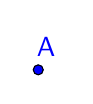
\begin{tikzpicture}[scale = 2]
	\draw
	(0,0) coordinate(A)
	(0.05,0.025) coordinate(pos)
	node[blue, anchor = south] {$\mathsf{A}$}  
	[blue,fill](A) circle(0.85pt); 
	\draw      [color = black](A) circle(0.9pt);
	\end{tikzpicture}
}
\newcommand{\Linustrik}{%  Strik, segment
	
\begin{tikzpicture}[scale = 0.4]
	\draw
	(0,0) coordinate(A)
	(1,0.7) coordinate(B)
	[line width = 1pt, blue](A)--(B);
	\draw[blue, fill](A) circle(4pt);
	\draw[blue, fill](B) circle(4pt);
	\end{tikzpicture}	
}

\newcommand{\Lina}{% bein lína, hægt að framlengja að vild
	
\begin{tikzpicture}[scale = 0.5]
	\draw
	(0,0) coordinate(A)
	(1,0.7) coordinate(B)
	[line width = 1pt, blue](A)--(B);
	\draw[blue, fill](0.25,0.18) circle(3pt);
	\draw[blue, fill](0.74,0.53) circle(3pt);
	\end{tikzpicture}	
}
\newcommand{\Halflina}{% við smíð á hornum
	
\begin{tikzpicture}[scale = 0.4]
	\draw
	(0,0) coordinate(A)
	(1,0.7) coordinate(B)
	[line width = 1pt, blue](A)--(B);
	\draw[blue, fill](A) circle(3pt);
	\draw[blue, fill](0.65,0.45) circle(3pt);
	\end{tikzpicture}	
	
}

\newcommand{\GeoO}{
	\begin{tikzpicture}[rotate=30,transform canvas={scale=0.18},yshift=7mm]
	\def\xrad{0.7}
	\def\yrad{0.58}
	\definecolor{GeogebraLitur}{rgb}{0.6,0.60,100}
	\tikzset{hnutur/.style={shape=circle, line width=0.7mm,color=black, fill=GeogebraLitur, scale=0.8, draw}} % 0.8
	\draw[ color = gray!70!black, line width=1.3mm] (0,0) circle[x radius = \xrad cm, y radius = \yrad cm];
	\def\n{5}
	\foreach \k in {1,...,\n}
	\node at ({360/\n*\k-10}:\xrad cm and \yrad cm)[hnutur] {};
	%	node[pos=1,hnutur]{} ;
	\end{tikzpicture}
}
\newcommand{\Geogebra}{{\color{gray!70!black}\textsf{Ge}\ \GeoO\textsf{Gebra }}}


%%%%%%%%%%%%%%%%%%%%%%%%%% Hyperlink References %%%%%%%%%%%%%%%%%%%%%%%%%%%
\usepackage{hyperref}

%--------------------% Storage Path for images %-----------------%
\graphicspath{{graphics/}{Graphics/}{./}}